%!TEX root = ../paper.tex
\section{Video Classification in Caffe}
\label{sec:classification}

For building our artificial neural network we used the Caffe\footnote{\url{http://caffe.berkeleyvision.org/}} framework.
Caffe is a deep learning framework offering several implementations of common layers.
The source code for Caffe is hosted on GitHub available to be adapted and extended for special use cases.
We worked with the Caffe branch of Jeff Donahue\footnote{\url{https://github.com/BVLC/caffe/pull/2033}}, which offers an implementation for long-short-term memory (LSTM) networks.

Wu at al \cite{wu2015modeling} proposed a hybrid deep learning for video classification resulting in a complex artificial neural network architecture.
It comprises of three components: the \emph{spatial}, \emph{flow} and \emph{fusion} nets respectively.

The \emph{spatial} part is processing the single frames of a video in order to recognize objects and structures in frames.
The \emph{flow} part memorizes motion of actions by learning the optical flow images.
Both parts consist of a convolutional neural network (CNN) followed by a long-short-term memory (LSTM) recurrent neural network (RNN).
To merge the predictions of both parts, \emph{spatial} and \emph{flow}, a third part is introduced.
This part, called \emph{fusion}, takes the output of both CNNs and merges their predictions.
Hence the final overall prediction is a combination of the three results.

% COMMENT: Wir haben das nur mäßig getestet und damals gab es glaube auch noch die ein oder andere Unstimmigkeit in den Daten, aber damals haben wir ein eher mäßige Verbesserung von 1% oder so bekommen, während das entsprechende Paper deutlich mehr versprochen hatte, oder so...
Our initial test indicated that the use of LSTMs did not improve our prediction results.
Therefore we eliminated the LSTM parts for our network structure, leaving us more in line with two-stream approach of Simonyan et al\cite{simonyan2014two}, as shown in Figure~\ref{fig:architecture}.
The simplified approach retains a separate CNN's for spatial and flow as well as the fusion network.

\begin{figure}[!htb]
	\centering
	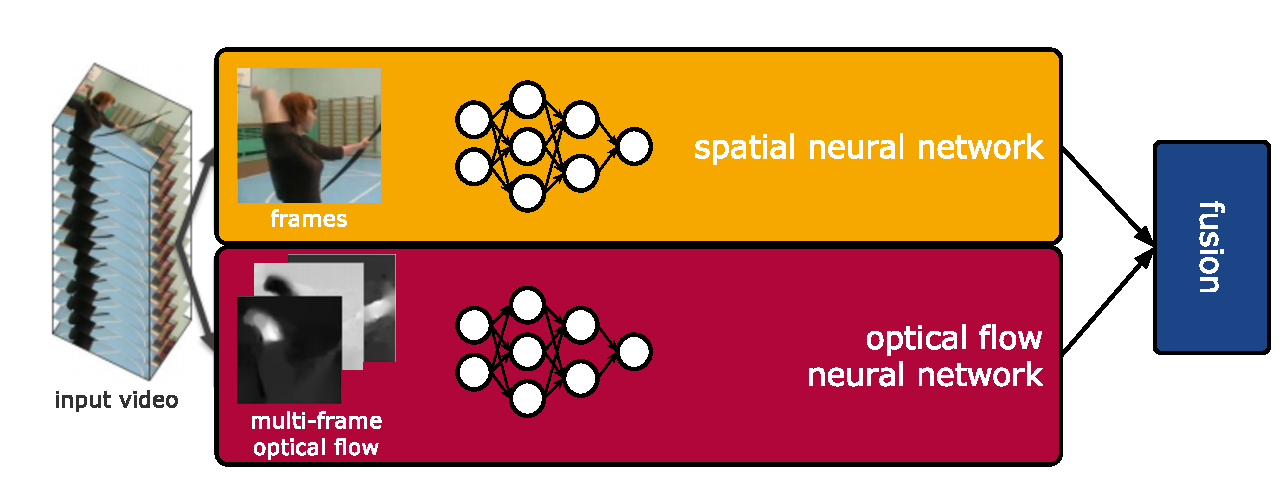
\includegraphics[scale=.7]{images/net_architecture.eps}
	\caption{Our neural network architecture consisting of three components: \emph{spatial}, \emph{flow} and \emph{fusion}. The \emph{spatial} and \emph{flow} neural network are convolutional neural networks. The predictions of both networks are combined in the third \emph{fusion} network.}
	\label{fig:architecture}
\end{figure}

During our research we tried out different neural networks, which will be presented in this section.
Additionally, we will summarize the results and hyperparameters, which were used for the training.

\subsection{Modifications to Caffe}

Working with a neural network consisting of LSTMs requires two different inputs:
On the one hand the raw pixel values and on the other hand a binary tagging sequence.
The tagging sequence tells the LSTM, where a new training example starts.
This is important, as there is more than one training sequence per batch.
A tagging sequence consist of 0's and 1's.
A 1 indicates the beginning of a new sequence.
For generating this tagging sequence we wrote a new data-generation strategy for the \emph{DummyData} layer.
This layer is meant to generate artificial data: Existing implementations generate constant values, uniformly distributed and gaussian distributed data etc.

An example of the dummy data layer can be found in Listing~\ref{lst:seq-layer}.
The layer has the following two parameters:
The \texttt{shape} parameter defines the output shape of the tagging blob, i.e. \texttt{16 x 4} in the example.
The second parameter \texttt{data\_filler} sets the concrete parameters for the dummy data.
In our case, we specify the tagging sequence data generation type.
The parameter \texttt{value} specifies the length of a sequence.
In the example, this means that there is single one, followed by 15 zeroes.

\begin{lstlisting}[language=sh, caption=Sequence Layer, label=lst:seq-layer]
layer {
	name: "sequence"
	type: "DummyData"
	top: "sequence"
	dummy_data_param {
		shape {
			dim: 16
			dim: 4
		}
		data_filler {
			type: "sequence"
			value: 16
		}
	}
}
\end{lstlisting}

In order to create stacked optical flow data we made a second modification to Caffe.
As mentioned in section \ref{subsec:convert_imageset_multi}, we added a utility script to bundle a list of images into a database of stacked images.

\subsection{Experiment infrastructure}
For running experiments with different parameter settings, we build a script, which helps with keeping track of different experiments.
It can be found in the \texttt{nets/*} subfolders under the name \texttt{train.sh}.
It is started like \texttt{train.sh dropout0.7fps30}, where the parameter indicates the name of the experiment.
This automatically creates a folder \texttt{experiments/20150907-100235\_dropout0.7fps30}, where the first numbers indicate the date and time of the experiment.
Before starting the experiment in Caffe, the script automatically copies the net and solver definitions to this folder.
After the training has finished or has been aborted, it copies the logs and the latest snapshots to the same folder.
It also automatically parses the logs and creates charts, which plot the iteration number against training loss, learning rate and test accuracy.
We used this script for all of our experiments and think it is of great value.

\subsection{Spatial}
\label{subsec:spatial}


\begin{table}[H]
\centering
\caption{Spatial Net Configurations}
\label{table:spatial_results}
\begin{tabularx}{\textwidth}{XXXXXXXX}
\toprule
Net 		& Layers	& Accuracy	& Learning Rate 	& Dropout Rate	& Finetuned Layers	& Iterations	& FPS\\ \midrule
CNN\_M		& 8			& 80\%		& 0.001			 	& 0.5			& 3					& 100.000		& 15\\
\bottomrule
\end{tabularx}
\end{table}


\begin{itemize}
	\item
		Different nets:
		\begin{itemize}
			\item Caffenet/CNN\_M (also tried, VGG 19, but too big)
			\item With weights/without weights
			\item Compare the nets with respect to memory, number of parameters, training time, performance
		\end{itemize}
	\item
		Experiments:
		\begin{itemize}
			\item Different dropouts
			\item Train from scratch vs train from weights
			\item On different splits?
			\item Fc6, Fc7, fc8
			\item Different base data sets (only 16, all data)
			\item Different flows?
			\item Occlusion tests
		\end{itemize}
	\item
		LSTM did not work out
\end{itemize}


\subsection{Flow}
\label{subsec:flow}

\begin{table}[H]
\centering
\caption{Flow Net Configurations}
\label{table:flow_results}
\begin{tabularx}{\textwidth}{XXXXXXXX}
\toprule
Net 		& Layers	& Accuracy	& Learning Rate 	& Dropout Rate	& Finetuned Layers	& Iterations	& FPS\\ \midrule
CNN\_M		& 8			& 80\%		& 0.001			 	& 0.5			& 3					& 100.000		& 15\\
\bottomrule
\end{tabularx}
\end{table}

\subsection{Fusion}
\label{subsec:fusion}

To combine the respective results from \emph{spatial} and \emph{flow} we need a third component.
For the fusion part we can use an additional machine learning algorithm to further generalize our prediction results.
To establish a baseline, we applied a support vector machine (SVM) for the fusion.
We followed up by using neutral networks for the fusion.
In the following section we will present and evaluate different network configurations.


\begin{table}[H]
\centering
\caption{Fusion Net Configurations}
\label{table:fusion_results}
\begin{tabularx}{\textwidth}{XXXXXXXX}
\toprule
Net 		& Layers	& Accuracy	& Learning Rate 	& Dropout Rate	& Finetuned Layers	& Iterations	& FPS\\ \midrule
CNN\_M		& 8			& 80\%		& 0.001			 	& 0.5			& 3					& 100.000		& 15\\
\bottomrule
\end{tabularx}
\end{table}


\subsubsection{Support Vector Machine}
To establish a baseline we applied a SVM to the respective \emph{spatial} and \emph{flow} output.
its own.
\todo[inline]{Joseph}
This approach resulted in fusion accuracy of 75\%, barely better than the \emph{flow} network on

\subsubsection{Early Fusion}
Our \emph{early fusion} architecture was build on the fusion architecture presented by \todo[inline]{TODO (Wu et al?}.
We took the CNN\_Ms for \emph{spatial} and \emph{flow} presented above and build a fusion architecture on top of them.
We selected 16 frames per video as described in Section~\ref{sec:data} and pass them on to the CNNs for \emph{spatial} and \emph{flow}.
The CNNs were cut off after the \textit{fc6}-layer resulting in an output of 1 x 4096 per frame.
Having 16 frames in total this corresponds to an input of 16 x 4096 for both \emph{spatial} and \emph{flow} for the fusion net.
The first step in the fusion network is to merge the 16 predictions of one video into one overall prediction for the whole video for both \emph{spatial} and \emph{flow}.
This is done by taking the average prediction.
A fully-connected layer is then trained with those predictions before we concatenate the predictions of \emph{spatial} and \emph{flow}.
Finally two fully-connected layers are trained on the merged predictions.
The output is defined by an accuracy layer.
The whole architecture is shown in Figure~\ref{fig:early_fusion}.

\begin{figure}[!htb]
	\centering
	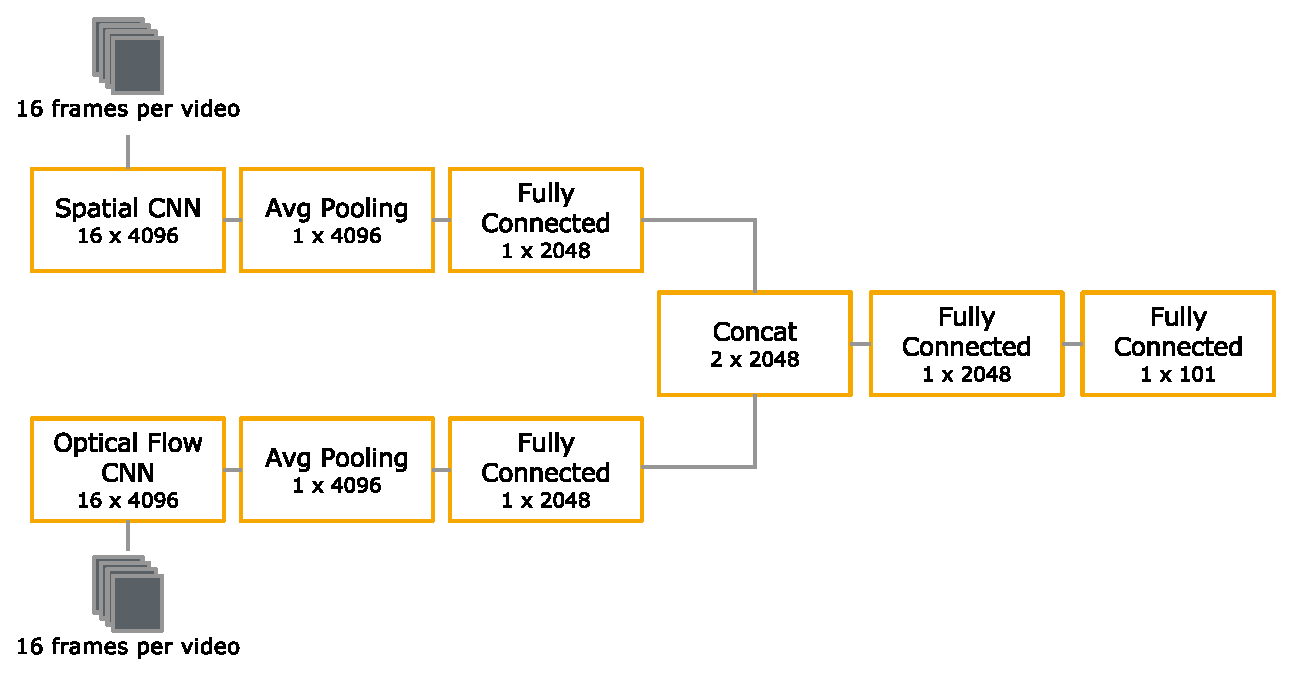
\includegraphics[scale=.7]{images/early_fusion.eps}
	\caption{Early fusion architecture: The predictions per frame of one video from the spatial and flow net are merged into one overall prediction per video each. Those predictions are then merged and trained via two fully connected layers.}
	\label{fig:early_fusion}
\end{figure}

\todo[inline]{TODO: results and parameter we tried}

\subsubsection{Middle Fusion}


\subsubsection{Late Fusion}


\begin{figure}[!htb]
	\centering
	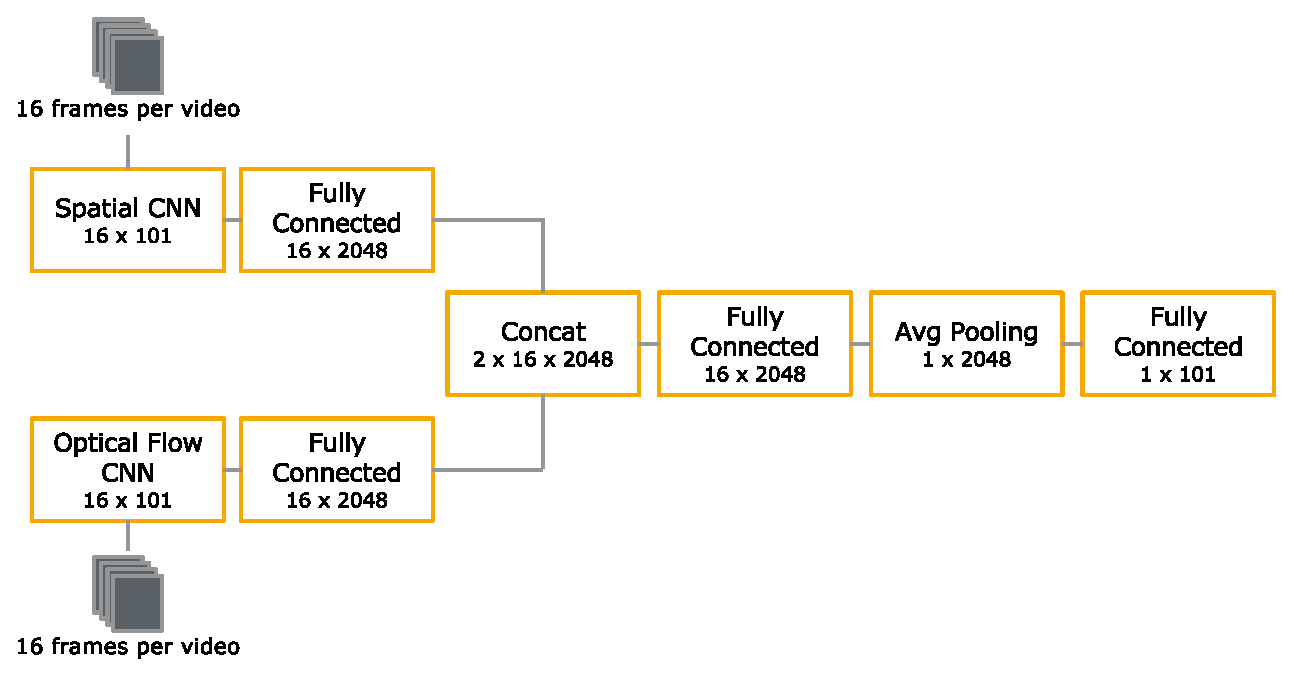
\includegraphics[scale=.7]{images/late_fusion.eps}
	\caption{}
	\label{fig:late_fusion}
\end{figure}